\documentclass[a4paper]{article}
\usepackage[a4paper,margin=0mm]{geometry}
\usepackage{fontspec}
\usepackage{unicode-math}
\usepackage{tikz}
\usepackage[table]{xcolor}
\usepackage[absolute]{textpos}
\usepackage{enumitem}
\usepackage{array}
\usepackage{multirow}

\setmainfont{Libertinus Serif}
\setsansfont{Libertinus Sans}
\setmathfont{Libertinus Math}
\newfontfamily\trackedsans{Libertinus Sans}[LetterSpace=8.0]

\definecolor{accent}{HTML}{F46530}
\definecolor{badge}{HTML}{FFBDA5}
\definecolor{ink}{HTML}{2A2E30}

\setlength{\TPHorizModule}{1mm}
\setlength{\TPVertModule}{1mm}
\setlength{\parindent}{0pt}
\pagestyle{empty}

\newcommand{\LCOL}{16mm}
\newcommand{\RCOL}{111mm}
\newcommand{\COLW}{83mm}

\newcommand{\topicheader}[2]{%
\begin{textblock*}{194mm}(16mm,10mm)
\begin{tikzpicture}
\node[fill=accent,text=white,font=\sffamily\bfseries\fontsize{13}{13}\selectfont,
      minimum width=9mm,minimum height=9mm,inner sep=0pt] at (4.5mm,-4.5mm) {#1};
\node[font=\sffamily\bfseries\fontsize{15}{16}\selectfont,text=ink,anchor=west] at (12mm,-4.5mm) {#2};
\end{tikzpicture}
\end{textblock*}
\begin{textblock*}{194mm}(16mm,22.5mm)

\begin{tikzpicture}
\fill[accent] (0,0) rectangle (194mm,0.5mm);
\end{tikzpicture}
\end{textblock*}
}

\newcommand{\pagefooter}[1]{%
\begin{textblock*}{194mm}(8mm,286.41mm)
  
\begin{tikzpicture}
    \fill[accent] (0,0) rectangle (194mm,0.6mm);
  \end{tikzpicture}
\end{textblock*}
\begin{textblock*}{63.59mm}(8mm,288.27mm)
  {\sffamily\bfseries\color{accent}\fontsize{13}{16}\selectfont SAT 1200+}
\end{textblock*}
\begin{textblock*}{10mm}(188mm,288.27mm)
  \centering{\sffamily\color{accent}\fontsize{14}{16}\selectfont #1}
\end{textblock*}
}

\newcommand{\colrule}[2]{%
\begin{textblock*}{1mm}(105mm,#1mm)
\begin{tikzpicture}
\draw[black!65,line width=0.5pt] (0,0) -- (0,#2mm);
\end{tikzpicture}
\end{textblock*}
}

\newcommand{\setkicker}[2]{%
{\sffamily\bfseries\fontsize{12}{14}\selectfont #1.}\ {\itshape\fontsize{11}{14}\selectfont\color{black!75} #2}\par\vspace{2mm}%
}

\setlength{\fboxsep}{1.4pt}
\setlength{\fboxrule}{0.5pt}
\newcommand{\pnum}[1]{\fcolorbox{ink}{white}{\sffamily\bfseries\fontsize{8}{8}\selectfont #1}~}

\newcommand{\qrbox}[1]{%
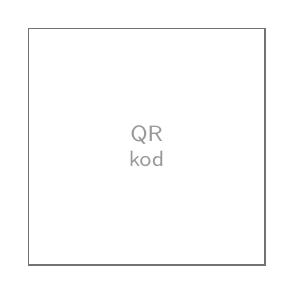
\begin{tikzpicture}
\draw[black!55,line width=0.6pt] (0,0) rectangle (30mm,30mm);
\node[black!40,font=\sffamily\fontsize{8}{9}\selectfont,align=center] at (15mm,15mm) {QR\\kod};
\end{tikzpicture}\\[1.5mm]
{\sffamily\fontsize{9}{11}\selectfont\color{black!70} #1}%
}

% ---- SAT-style multiple-choice question block: #1=number #2=stem #3-6=choices A-D ----
\newcommand{\satq}[6]{%
\noindent\pnum{#1} #2\\[2mm]
\hspace*{7mm}\begin{tabular}{@{}p{32mm}p{32mm}@{}}
(A) #3 & (B) #4 \\[2.5mm]
(C) #5 & (D) #6 \\
\end{tabular}\\[7mm]%
}

\arrayrulecolor{accent}
\setlength{\arrayrulewidth}{0.7pt}
\renewcommand{\arraystretch}{1.35}
\newcommand{\anstitle}[1]{{\sffamily\bfseries\color{accent}\fontsize{11}{13}\selectfont #1}\\[1.3mm]}

\begin{document}

% ================= PAGE 1: Set 1 | Set 2 =================
\topicheader{5}{ALGEBRAIK IFODALAR}
\pagefooter{39}
\colrule{32}{238}
\mbox{}%

\begin{textblock*}{\COLW}(\LCOL,32mm)
{\fontsize{12}{15}\selectfont
\setkicker{1-to'plam}{O'xshash hadlarni qo'shing (musbat koeffitsientlar).}

\noindent\pnum{1} $3x+5x=$\\[22mm]
\noindent\pnum{2} $7y+2y+y=$\\[22mm]
\noindent\pnum{3} $4a+3b+2a=$\\[22mm]
\noindent\pnum{4} $6x+3+2x=$\\[22mm]
\noindent\pnum{5} $5m+4n+3m+n=$\\[22mm]
\noindent\pnum{6} $2x+3x+4x=$\\[22mm]
\noindent\pnum{7} $8p+5q+2p+3q=$\\[22mm]
\noindent\pnum{8} $x+x+x+x=$
}
\end{textblock*}

\begin{textblock*}{\COLW}(\RCOL,32mm)
{\fontsize{12}{15}\selectfont
\setkicker{2-to'plam}{O'xshash hadlarni qo'shing -- ayirish ishtirok etadi.}

\noindent\pnum{1} $7x-3x=$\\[22mm]
\noindent\pnum{2} $5a-8a=$\\[22mm]
\noindent\pnum{3} $4x-7+2x=$\\[22mm]
\noindent\pnum{4} $-3y+5y-2y=$\\[22mm]
\noindent\pnum{5} $6m-4n-2m+7n=$\\[22mm]
\noindent\pnum{6} $-5x+3x-8=$\\[22mm]
\noindent\pnum{7} $2a-5a+6a=$\\[22mm]
\noindent\pnum{8} $9x-4x-x=$
}
\end{textblock*}

\clearpage

% ================= PAGE 2: Set 3 | Set 4 =================
\topicheader{5}{ALGEBRAIK IFODALAR}
\pagefooter{40}
\colrule{32}{238}
\mbox{}%

\begin{textblock*}{\COLW}(\LCOL,32mm)
{\fontsize{12}{15}\selectfont
\setkicker{3-to'plam}{Taqsimot qonunini qo'llang (musbat ko'paytuvchi).}

\noindent\pnum{1} $3(x+4)=$\\[22mm]
\noindent\pnum{2} $5(2x-3)=$\\[22mm]
\noindent\pnum{3} $2(3a+4b)=$\\[22mm]
\noindent\pnum{4} $4(x-1)=$\\[22mm]
\noindent\pnum{5} $6(2+3x)=$\\[22mm]
\noindent\pnum{6} $7(x+y)=$\\[22mm]
\noindent\pnum{7} $3(4x-2)=$\\[22mm]
\noindent\pnum{8} $2(5x+3)=$
}
\end{textblock*}

\begin{textblock*}{\COLW}(\RCOL,32mm)
{\fontsize{12}{15}\selectfont
\setkicker{4-to'plam}{Taqsimot qonuni -- manfiy ko'paytuvchini har bir hadga tarqating.}

\noindent\pnum{1} $-2(x+3)=$\\[22mm]
\noindent\pnum{2} $-(3x-5)=$\\[22mm]
\noindent\pnum{3} $-4(2x-1)=$\\[22mm]
\noindent\pnum{4} $-(x+7)=$\\[22mm]
\noindent\pnum{5} $-3(4-x)=$\\[22mm]
\noindent\pnum{6} $-(2x-3y)=$\\[22mm]
\noindent\pnum{7} $-5(x+2)=$\\[22mm]
\noindent\pnum{8} $-(-x+4)=$
}
\end{textblock*}

\clearpage

% ================= PAGE 3: Set 5 | Set 6 (spot the error) =================
\topicheader{5}{ALGEBRAIK IFODALAR}
\pagefooter{41}
\colrule{32}{238}
\mbox{}%

\begin{textblock*}{\COLW}(\LCOL,32mm)
{\fontsize{12}{15}\selectfont
\setkicker{5-to'plam}{Aralash -- avval taqsimlang, so'ng o'xshash hadlarni qo'shing.}

\noindent\pnum{1} $3(x+2)+4x=$\\[22mm]
\noindent\pnum{2} $5(2x-1)-3x=$\\[22mm]
\noindent\pnum{3} $2(x+3)-(x-1)=$\\[22mm]
\noindent\pnum{4} $4(x-2)+3(x+1)=$\\[22mm]
\noindent\pnum{5} $-(2x+3)+5x=$\\[22mm]
\noindent\pnum{6} $3(x-1)-2(x+2)=$\\[22mm]
\noindent\pnum{7} $2(3x+1)-(4x-5)=$\\[22mm]
\noindent\pnum{8} $5-2(x-3)=$
}
\end{textblock*}

\begin{textblock*}{\COLW}(\RCOL,32mm)
{\fontsize{11}{14}\selectfont
\setkicker{6-to'plam}{Xatoni toping -- buzilgan qadamni ayting, to'g'ri soddalashtirilgan ko'rinishni bering.}

\noindent\pnum{1} $-(3x-5)$ ifodasini soddalashtirishda ko'rsatilgan yechimda xato bor:\\[1mm]
\hspace*{7mm}\textit{``$-3x-5$''}\\[2mm]
\hspace*{7mm}Xato va to'g'ri javob: \makebox[52mm]{\dotfill}\\[10mm]

\noindent\pnum{2} $4x+3x^2$ ifodasini soddalashtirishda ko'rsatilgan yechimda xato bor:\\[1mm]
\hspace*{7mm}\textit{``$7x^2$''}\\[2mm]
\hspace*{7mm}Xato va to'g'ri javob: \makebox[52mm]{\dotfill}\\[10mm]

\noindent\pnum{3} $-2(x-4)$ ifodasini soddalashtirishda ko'rsatilgan yechimda xato bor:\\[1mm]
\hspace*{7mm}\textit{``$-2x-8$''}\\[2mm]
\hspace*{7mm}Xato va to'g'ri javob: \makebox[52mm]{\dotfill}\\[10mm]

\noindent\pnum{4} $5x-(2x-3)$ ifodasini soddalashtirishda ko'rsatilgan yechimda xato bor:\\[1mm]
\hspace*{7mm}\textit{``$5x-2x-3=3x-3$''}\\[2mm]
\hspace*{7mm}Xato va to'g'ri javob: \makebox[52mm]{\dotfill}\\[10mm]

\noindent\pnum{5} $3(2x+1)-4$ ifodasini soddalashtirishda ko'rsatilgan yechimda xato bor:\\[1mm]
\hspace*{7mm}\textit{``$6x+1-4=6x-3$''}\\[2mm]
\hspace*{7mm}Xato va to'g'ri javob: \makebox[52mm]{\dotfill}
}
\end{textblock*}

\clearpage

% ================= PAGE 4: Set 7 (bonus, left) + Set 8 pt.1 (right) -- no dead column =================
\topicheader{5}{ALGEBRAIK IFODALAR}
\pagefooter{42}
\colrule{32}{238}
\mbox{}%

\begin{textblock*}{\COLW}(\LCOL,32mm)
{\fontsize{12}{15}\selectfont
\setkicker{7-to'plam}{Bonus / qiyin -- ichma-ich qavslar va ikki o'zgaruvchili ifodalar.}

\noindent\pnum{1} $2\left[3(x+1)-2x\right]+5=$\\[26mm]
\noindent\pnum{2} $-3(x-2)+2(x+4)-5=$\\[26mm]
\noindent\pnum{3} $4x-2\left[x-(3x+1)\right]=$\\[26mm]
\noindent\pnum{4} $5(a-2b)-3(2a-b)=$\\[26mm]
\noindent\pnum{5} $-\left[2(x+3)-(x-1)\right]+4x=$
}
\end{textblock*}

\begin{textblock*}{\COLW}(\RCOL,32mm)
{\fontsize{10.5}{13}\selectfont
\setkicker{8-to'plam}{SAT'da qanday uchraydi -- had, koeffitsient va teng kuchli ifodalar.}

\satq{1}{$7x-4y+9$ ifodasida $y$ ning koeffitsienti nechaga teng?}{4}{$-4$}{7}{9}
\satq{2}{$5x+3-2x+8$ ifodasiga teng ifodani toping.}{$3x+11$}{$7x+11$}{$3x+5$}{$7x+5$}
\satq{3}{$4(2x-3)$ ifodasiga teng ifodani toping.}{$8x-3$}{$6x-12$}{$2x-12$}{$8x-12$}
\satq{4}{$-3(x-5)$ ifodasiga teng ifodani toping.}{$-3x-5$}{$-3x-15$}{$-3x+15$}{$3x-15$}
\satq{5}{$6x+2(x-3)$ ifodasiga teng ifodani toping.}{$8x-3$}{$6x+1$}{$8x+6$}{$8x-6$}
\satq{6}{To'rtburchakning eni $x$, uzunligi esa enidan ikki baravar ortiq va yana $3$ birlik ko'p. Perimetri uchun qaysi ifoda to'g'ri?}{$3x+3$}{$6x+6$}{$6x+3$}{$3x+6$}
}
\end{textblock*}

\clearpage

% ================= PAGE 5: Set 8 pt.2 (continues directly, no title page of its own) =================
\topicheader{5}{ALGEBRAIK IFODALAR}
\pagefooter{43}
\colrule{32}{238}
\mbox{}%

\begin{textblock*}{\COLW}(\LCOL,32mm)
{\fontsize{10.5}{13}\selectfont
\satq{7}{$2(3x+4)-(x-5)$ ifodasiga teng ifodani toping.}{$5x+3$}{$5x-13$}{$5x+13$}{$7x+13$}
\satq{8}{Do'konda daftar narxi \$3, xaridda bir martalik \$5 chegirma beriladi. $n$ ta daftar uchun jami narx (dollarda) qanday ifoda bilan beriladi?}{$3n+5$}{$3(n-5)$}{$5n-3$}{$3n-5$}
\satq{9}{$-2(3x-1)+4x$ ifodasiga teng ifodani toping.}{$2x+2$}{$-2x+2$}{$-2x-2$}{$10x+2$}
\satq{10}{$8-5x+2x^2$ ifodasida erkin had nechaga teng?}{8}{$-5x$}{$2x^2$}{$-5$}
\satq{11}{$3x+7-(x+7)$ ifodasiga teng ifodani toping.}{$2x+14$}{$4x$}{$2x-14$}{$2x$}
\satq{12}{Telefon tarifi oyiga \$15 + har gigabayt uchun \$2. $g$ gigabayt uchun jami narx (dollarda) qanday ifoda bilan beriladi?}{$15g+2$}{$2g-15$}{$2g+15$}{$17g$}
}
\end{textblock*}

\clearpage

% ================= PAGE 6: Qaydlar (notes) -- ruled writing space + video QR codes =================
\topicheader{5}{ALGEBRAIK IFODALAR}
\pagefooter{44}
\mbox{}%

\begin{textblock*}{194mm}(16mm,34mm)
{\bfseries\itshape\color{accent}\fontsize{19}{21}\selectfont\centering Qaydlar uchun\par}
\end{textblock*}

\begin{textblock*}{194mm}(16mm,46mm)
{\fontsize{11}{14}\selectfont\color{black!65}\centering\itshape Nimalar esingizda qoldi?\par}
\end{textblock*}

\begin{textblock*}{178mm}(16mm,62mm)
\begin{tikzpicture}
\foreach \y in {0,13,...,169}{
  \draw[black!25,line width=0.5pt] (0,-\y mm) -- (178mm,-\y mm);
}
\end{tikzpicture}
\end{textblock*}

\begin{textblock*}{194mm}(16mm,240mm)
\centering
{\sffamily\fontsize{9.5}{11.5}\selectfont\color{black!70} Video yechimlar va qo'shimcha testlar uchun quyidagi QR kodlarni skanerlang:}\\[4mm]
\begin{minipage}[t]{32mm}\centering\qrbox{YouTube}\end{minipage}%
\hspace{16mm}%
\begin{minipage}[t]{32mm}\centering\qrbox{Telegram}\end{minipage}
\end{textblock*}

\clearpage

% ================= PAGE 7: Javoblar -- full-page unified answer table =================
\topicheader{5}{ALGEBRAIK IFODALAR}
\pagefooter{45}
\mbox{}%

\begin{textblock*}{194mm}(16mm,30mm)
{\bfseries\itshape\color{accent}\fontsize{19}{21}\selectfont\centering Javoblar\par}
\end{textblock*}

\begin{textblock*}{194mm}(16mm,44mm)
{\fontsize{10}{12.5}\selectfont
\centering
\renewcommand{\arraystretch}{1.15}
\begin{tabular}{|>{\centering\arraybackslash}p{26mm}|>{\centering\arraybackslash}p{10mm}|>{\centering\arraybackslash}p{36mm}|>{\centering\arraybackslash}p{10mm}|>{\centering\arraybackslash}p{36mm}|}
\hline
\rowcolor{badge!55}\textbf{To'plam} & \textbf{\#} & \textbf{Javob} & \textbf{\#} & \textbf{Javob}\\
\hline
\multirow{4}{26mm}{\centering 1-to'plam} & 1 & $8x$ & 2 & $10y$\\\cline{2-5}
 & 3 & $6a+3b$ & 4 & $8x+3$\\\cline{2-5}
 & 5 & $8m+5n$ & 6 & $9x$\\\cline{2-5}
 & 7 & $10p+8q$ & 8 & $4x$\\\hline
\multirow{4}{26mm}{\centering 2-to'plam} & 1 & $4x$ & 2 & $-3a$\\\cline{2-5}
 & 3 & $6x-7$ & 4 & $0$\\\cline{2-5}
 & 5 & $4m+3n$ & 6 & $-2x-8$\\\cline{2-5}
 & 7 & $3a$ & 8 & $4x$\\\hline
\multirow{4}{26mm}{\centering 3-to'plam} & 1 & $3x+12$ & 2 & $10x-15$\\\cline{2-5}
 & 3 & $6a+8b$ & 4 & $4x-4$\\\cline{2-5}
 & 5 & $18x+12$ & 6 & $7x+7y$\\\cline{2-5}
 & 7 & $12x-6$ & 8 & $10x+6$\\\hline
\multirow{4}{26mm}{\centering 4-to'plam} & 1 & $-2x-6$ & 2 & $5-3x$\\\cline{2-5}
 & 3 & $4-8x$ & 4 & $-x-7$\\\cline{2-5}
 & 5 & $3x-12$ & 6 & $-2x+3y$\\\cline{2-5}
 & 7 & $-5x-10$ & 8 & $x-4$\\\hline
\multirow{4}{26mm}{\centering 5-to'plam} & 1 & $7x+6$ & 2 & $7x-5$\\\cline{2-5}
 & 3 & $x+7$ & 4 & $7x-5$\\\cline{2-5}
 & 5 & $3x-3$ & 6 & $x-7$\\\cline{2-5}
 & 7 & $2x+7$ & 8 & $11-2x$\\\hline
\multirow{3}{26mm}{\centering 7-to'plam} & 1 & $2x+11$ & 2 & $9-x$\\\cline{2-5}
 & 3 & $8x+2$ & 4 & $-a-7b$\\\cline{2-5}
 & 5 & $3x-7$ & -- & --\\\hline
\multirow{6}{26mm}{\centering 8-to'plam} & 1 & B & 2 & A\\\cline{2-5}
 & 3 & D & 4 & C\\\cline{2-5}
 & 5 & D & 6 & B\\\cline{2-5}
 & 7 & C & 8 & D\\\cline{2-5}
 & 9 & B & 10 & A\\\cline{2-5}
 & 11 & D & 12 & C\\\hline
\multirow{5}{26mm}{\centering 6-to'plam} & \multicolumn{4}{p{92mm}|}{1.\ Xato -- manfiy ishora faqat $3x$ ga tarqatilgan, $-5$ ga emas. To'g'ri: $-(3x-5)=5-3x$.}\\\cline{2-5}
 & \multicolumn{4}{p{92mm}|}{2.\ Xato -- $x$ va $x^2$ o'xshash had emas (daraja boshqa), qo'shib bo'lmaydi. To'g'ri: $3x^2+4x$ (allaqachon sodda).}\\\cline{2-5}
 & \multicolumn{4}{p{92mm}|}{3.\ Xato -- $-2\times(-4)=+8$ bo'lishi kerak edi, ishora tushib qolgan. To'g'ri: $-2(x-4)=8-2x$.}\\\cline{2-5}
 & \multicolumn{4}{p{92mm}|}{4.\ Xato -- qavs oldidagi manfiy ishora faqat $2x$ ga tarqatilgan, $-3$ ga emas. To'g'ri: $5x-(2x-3)=3x+3$.}\\\cline{2-5}
 & \multicolumn{4}{p{92mm}|}{5.\ Xato -- $3\times1$ hisoblanmagan (ikkinchi hadga tarqatish o'tkazib yuborilgan). To'g'ri: $3(2x+1)-4=6x-1$.}\\\hline
\end{tabular}
}
\end{textblock*}

\end{document}
